\section{Identifying Posture}

The Biggest hurdle, was and still is identifying and correctly analysing the data. I have had several different aproaches on how to interpret and visualize the data. During my first attempt (Attemt A) i tried to visualized the data in two ways, with Python and Power BI.

Firstly I transformed the data into a CSV which is a commonly used format viable for many different applications

\subsection{Visualising with Python}

I tried to visualize the data using python since it was recommended on a few forums and seamed to be feasible for this task. It actually did work quite well and I have achieved within 2 Days with Python. I have never worked with python before and was happy that I managed to use and apply it within days. 

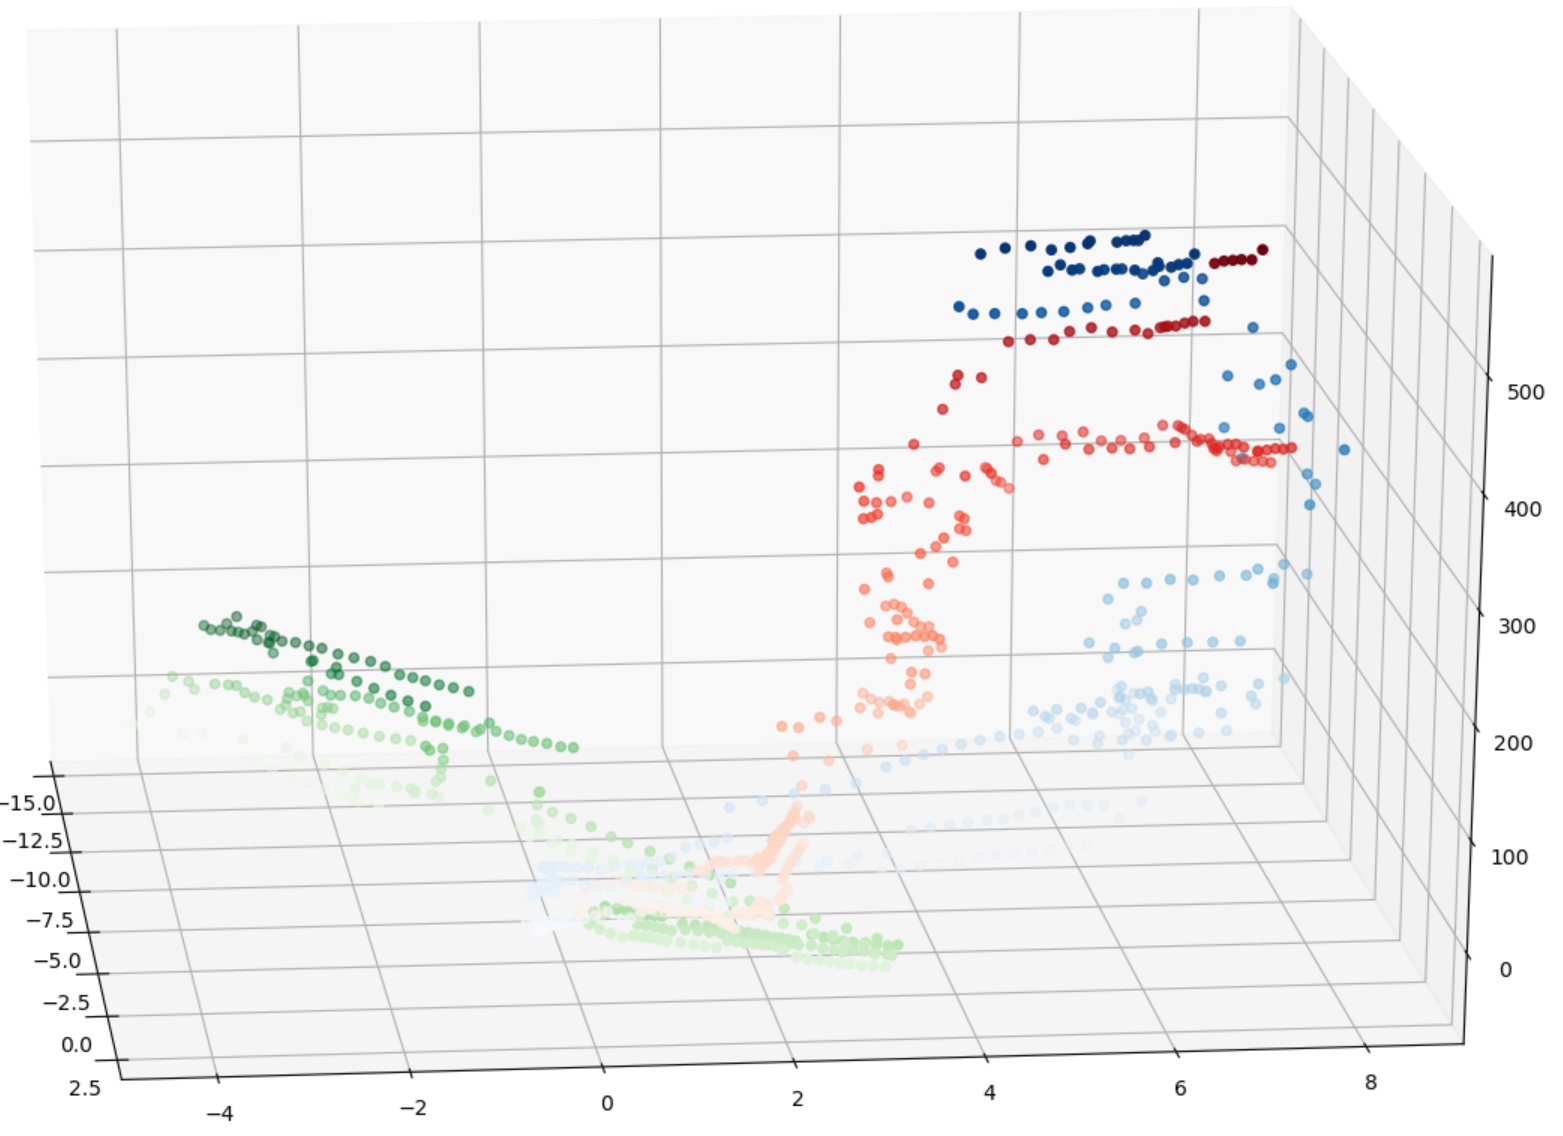
\includegraphics[width=\linewidth]{images/PyVisualisation.png}

Visualised you see my first attempt in showing movement of 3 sensors with the data of the accelometers. The sensors were attached to my shirt with scotch. This is not a perfect solution, which is visible in the different orientation of the green dots. 

Here I tried to add up the movement from the accelometers to see how this stacks up. The Data was not very helpful and i tried to anime the accelometer data directly to see how it changes, this was a bit clearer but still very hard to interpret since it was static data. 

To Visualize I used numpy and matplotlib which are quite handy but still took some time the get used to.
The data was simple display on a grapth (ax) from np arrays:

\begin{lstlisting}
ax.scatter3D(XSXAcc[:,0],XSXAcc[:,1],XSXAcc[:,2], c=XSXAcc[:,2], cmap='Reds')
ax.scatter3D(XSYAcc[:,0],XSYAcc[:,1],XSYAcc[:,2], c=XSYAcc[:,2], cmap='Blues')
ax.scatter3D(XSZAcc[:,0],XSZAcc[:,1],XSZAcc[:,2], c=XSZAcc[:,2], cmap='Greens')
\end{lstlisting}

\subsection{Visualising with Power BI}